\documentclass[1p]{elsarticle_modified}
%\bibliographystyle{elsarticle-num}

%\usepackage[colorlinks]{hyperref}
%\usepackage{abbrmath_seonhwa} %\Abb, \Ascr, \Acal ,\Abf, \Afrak
\usepackage{amsfonts}
\usepackage{amssymb}
\usepackage{amsmath}
\usepackage{amsthm}
\usepackage{scalefnt}
\usepackage{amsbsy}
\usepackage{kotex}
\usepackage{caption}
\usepackage{subfig}
\usepackage{color}
\usepackage{graphicx}
\usepackage{xcolor} %% white, black, red, green, blue, cyan, magenta, yellow
\usepackage{float}
\usepackage{setspace}
\usepackage{hyperref}

\usepackage{tikz}
\usetikzlibrary{arrows}

\usepackage{multirow}
\usepackage{array} % fixed length table
\usepackage{hhline}

%%%%%%%%%%%%%%%%%%%%%
\makeatletter
\renewcommand*\env@matrix[1][\arraystretch]{%
	\edef\arraystretch{#1}%
	\hskip -\arraycolsep
	\let\@ifnextchar\new@ifnextchar
	\array{*\c@MaxMatrixCols c}}
\makeatother %https://tex.stackexchange.com/questions/14071/how-can-i-increase-the-line-spacing-in-a-matrix
%%%%%%%%%%%%%%%

\usepackage[normalem]{ulem}

\newcommand{\msout}[1]{\ifmmode\text{\sout{\ensuremath{#1}}}\else\sout{#1}\fi}
%SOURCE: \msout is \stkout macro in https://tex.stackexchange.com/questions/20609/strikeout-in-math-mode

\newcommand{\cancel}[1]{
	\ifmmode
	{\color{red}\msout{#1}}
	\else
	{\color{red}\sout{#1}}
	\fi
}

\newcommand{\add}[1]{
	{\color{blue}\uwave{#1}}
}

\newcommand{\replace}[2]{
	\ifmmode
	{\color{red}\msout{#1}}{\color{blue}\uwave{#2}}
	\else
	{\color{red}\sout{#1}}{\color{blue}\uwave{#2}}
	\fi
}

\newcommand{\Sol}{\mathcal{S}} %segment
\newcommand{\D}{D} %diagram
\newcommand{\A}{\mathcal{A}} %arc


%%%%%%%%%%%%%%%%%%%%%%%%%%%%%5 test

\def\sl{\operatorname{\textup{SL}}(2,\Cbb)}
\def\psl{\operatorname{\textup{PSL}}(2,\Cbb)}
\def\quan{\mkern 1mu \triangleright \mkern 1mu}

\theoremstyle{definition}
\newtheorem{thm}{Theorem}[section]
\newtheorem{prop}[thm]{Proposition}
\newtheorem{lem}[thm]{Lemma}
\newtheorem{ques}[thm]{Question}
\newtheorem{cor}[thm]{Corollary}
\newtheorem{defn}[thm]{Definition}
\newtheorem{exam}[thm]{Example}
\newtheorem{rmk}[thm]{Remark}
\newtheorem{alg}[thm]{Algorithm}

\newcommand{\I}{\sqrt{-1}}
\begin{document}

%\begin{frontmatter}
%
%\title{Boundary parabolic representations of knots up to 8 crossings}
%
%%% Group authors per affiliation:
%\author{Yunhi Cho} 
%\address{Department of Mathematics, University of Seoul, Seoul, Korea}
%\ead{yhcho@uos.ac.kr}
%
%
%\author{Seonhwa Kim} %\fnref{s_kim}}
%\address{Center for Geometry and Physics, Institute for Basic Science, Pohang, 37673, Korea}
%\ead{ryeona17@ibs.re.kr}
%
%\author{Hyuk Kim}
%\address{Department of Mathematical Sciences, Seoul National University, Seoul 08826, Korea}
%\ead{hyukkim@snu.ac.kr}
%
%\author{Seokbeom Yoon}
%\address{Department of Mathematical Sciences, Seoul National University, Seoul, 08826,  Korea}
%\ead{sbyoon15@snu.ac.kr}
%
%\begin{abstract}
%We find all boundary parabolic representation of knots up to 8 crossings.
%
%\end{abstract}
%\begin{keyword}
%    \MSC[2010] 57M25 
%\end{keyword}
%
%\end{frontmatter}

%\linenumbers
%\tableofcontents
%
\newcommand\colored[1]{\textcolor{white}{\rule[-0.35ex]{0.8em}{1.4ex}}\kern-0.8em\color{red} #1}%
%\newcommand\colored[1]{\textcolor{white}{ #1}\kern-2.17ex	\textcolor{white}{ #1}\kern-1.81ex	\textcolor{white}{ #1}\kern-2.15ex\color{red}#1	}

{\Large $\underline{12a_{0831}~(K12a_{0831})}$}

\setlength{\tabcolsep}{10pt}
\renewcommand{\arraystretch}{1.6}
\vspace{1cm}\begin{tabular}{m{100pt}>{\centering\arraybackslash}m{274pt}}
\multirow{5}{120pt}{
	\centering
	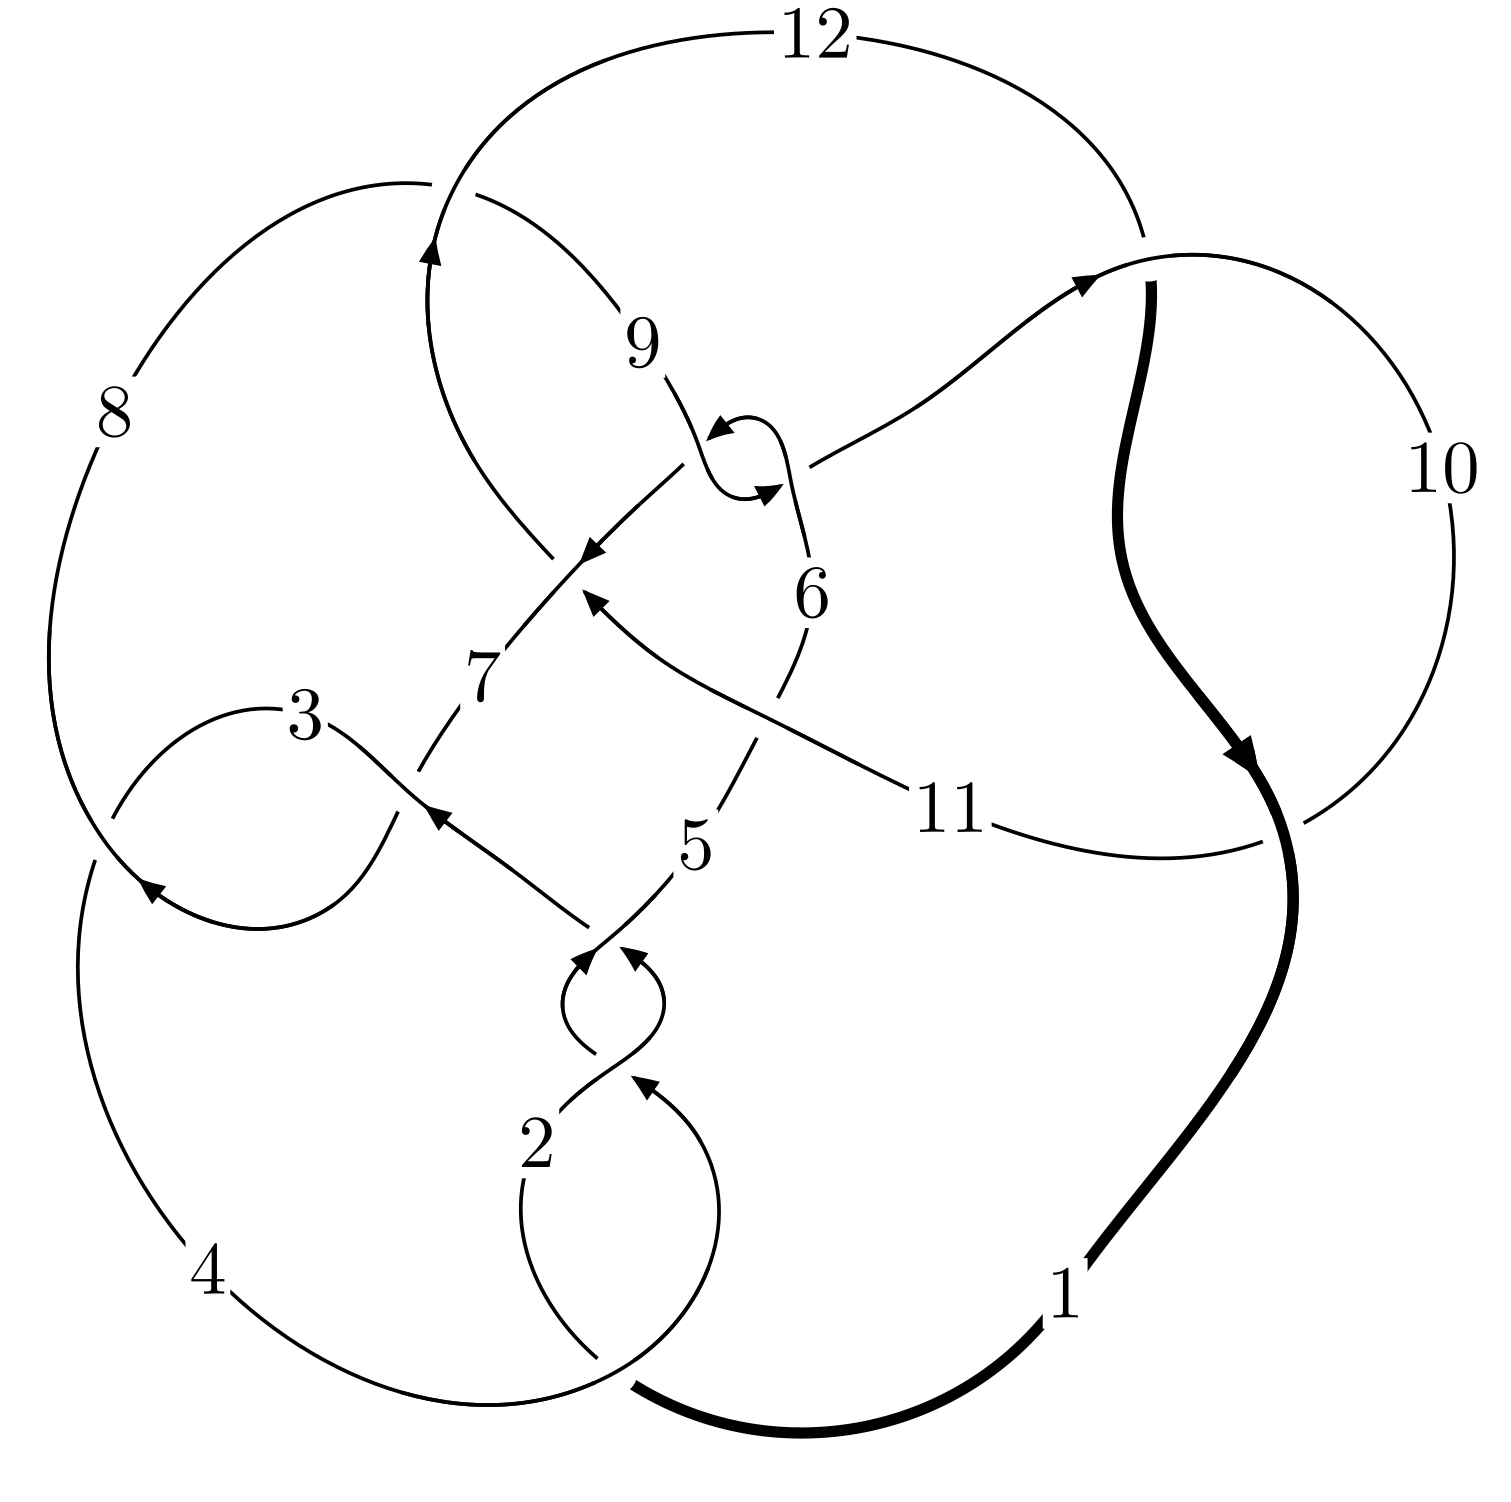
\includegraphics[width=112pt]{../../../GIT/diagram.site/Diagrams/png/1632_12a_0831.png}\\
\ \ \ A knot diagram\footnotemark}&
\allowdisplaybreaks
\textbf{Linearized knot diagam} \\
\cline{2-2}
 &
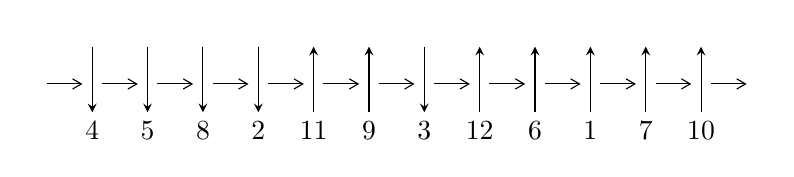
\begin{tikzpicture}[x=20pt, y=17pt]
	% nodes
	\node (C0) at (0, 0) {};
	\node (C1) at (1, 0) {};
	\node (C1U) at (1, +1) {};
	\node (C1D) at (1, -1) {4};

	\node (C2) at (2, 0) {};
	\node (C2U) at (2, +1) {};
	\node (C2D) at (2, -1) {5};

	\node (C3) at (3, 0) {};
	\node (C3U) at (3, +1) {};
	\node (C3D) at (3, -1) {8};

	\node (C4) at (4, 0) {};
	\node (C4U) at (4, +1) {};
	\node (C4D) at (4, -1) {2};

	\node (C5) at (5, 0) {};
	\node (C5U) at (5, +1) {};
	\node (C5D) at (5, -1) {11};

	\node (C6) at (6, 0) {};
	\node (C6U) at (6, +1) {};
	\node (C6D) at (6, -1) {9};

	\node (C7) at (7, 0) {};
	\node (C7U) at (7, +1) {};
	\node (C7D) at (7, -1) {3};

	\node (C8) at (8, 0) {};
	\node (C8U) at (8, +1) {};
	\node (C8D) at (8, -1) {12};

	\node (C9) at (9, 0) {};
	\node (C9U) at (9, +1) {};
	\node (C9D) at (9, -1) {6};

	\node (C10) at (10, 0) {};
	\node (C10U) at (10, +1) {};
	\node (C10D) at (10, -1) {1};

	\node (C11) at (11, 0) {};
	\node (C11U) at (11, +1) {};
	\node (C11D) at (11, -1) {7};

	\node (C12) at (12, 0) {};
	\node (C12U) at (12, +1) {};
	\node (C12D) at (12, -1) {10};
	\node (C13) at (13, 0) {};

	% arrows
	\draw[->,>={angle 60}]
	(C0) edge (C1) (C1) edge (C2) (C2) edge (C3) (C3) edge (C4) (C4) edge (C5) (C5) edge (C6) (C6) edge (C7) (C7) edge (C8) (C8) edge (C9) (C9) edge (C10) (C10) edge (C11) (C11) edge (C12) (C12) edge (C13) ;	\draw[->,>=stealth]
	(C1U) edge (C1D) (C2U) edge (C2D) (C3U) edge (C3D) (C4U) edge (C4D) (C5D) edge (C5U) (C6D) edge (C6U) (C7U) edge (C7D) (C8D) edge (C8U) (C9D) edge (C9U) (C10D) edge (C10U) (C11D) edge (C11U) (C12D) edge (C12U) ;
	\end{tikzpicture} \\
\hhline{~~} \\& 
\textbf{Solving Sequence} \\ \cline{2-2} 
 &
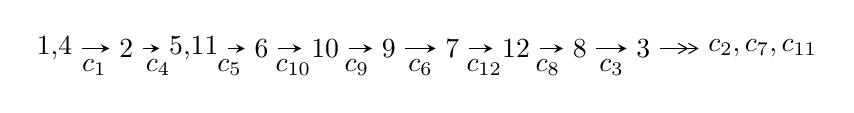
\begin{tikzpicture}[x=23pt, y=7pt]
	% node
	\node (A0) at (-1/8, 0) {1,4};
	\node (A1) at (1, 0) {2};
	\node (A2) at (33/16, 0) {5,11};
	\node (A3) at (25/8, 0) {6};
	\node (A4) at (33/8, 0) {10};
	\node (A5) at (41/8, 0) {9};
	\node (A6) at (49/8, 0) {7};
	\node (A7) at (57/8, 0) {12};
	\node (A8) at (65/8, 0) {8};
	\node (A9) at (73/8, 0) {3};
	\node (C1) at (1/2, -1) {$c_{1}$};
	\node (C2) at (3/2, -1) {$c_{4}$};
	\node (C3) at (21/8, -1) {$c_{5}$};
	\node (C4) at (29/8, -1) {$c_{10}$};
	\node (C5) at (37/8, -1) {$c_{9}$};
	\node (C6) at (45/8, -1) {$c_{6}$};
	\node (C7) at (53/8, -1) {$c_{12}$};
	\node (C8) at (61/8, -1) {$c_{8}$};
	\node (C9) at (69/8, -1) {$c_{3}$};
	\node (A10) at (11, 0) {$c_{2},c_{7},c_{11}$};

	% edge
	\draw[->,>=stealth]	
	(A0) edge (A1) (A1) edge (A2) (A2) edge (A3) (A3) edge (A4) (A4) edge (A5) (A5) edge (A6) (A6) edge (A7) (A7) edge (A8) (A8) edge (A9) ;
	\draw[->>,>={angle 60}]	
	(A9) edge (A10);
\end{tikzpicture} \\ 

\end{tabular} \\

\footnotetext{
The image of knot diagram is generated by the software ``\textbf{Draw programme}" developed by Andrew Bartholomew(\url{http://www.layer8.co.uk/maths/draw/index.htm\#Running-draw}), where we modified some parts for our purpose(\url{https://github.com/CATsTAILs/LinksPainter}).
}\phantom \\ \newline 
\centering \textbf{Ideals for irreducible components\footnotemark of $X_{\text{par}}$} 
 
\begin{align*}
I^u_{1}&=\langle 
-2.23861\times10^{153} u^{112}-1.94908\times10^{154} u^{111}+\cdots+1.41771\times10^{153} b-2.85035\times10^{153},\\
\phantom{I^u_{1}}&\phantom{= \langle  }-1.06042\times10^{155} u^{112}-1.06831\times10^{156} u^{111}+\cdots+2.41011\times10^{154} a-2.12527\times10^{155},\\
\phantom{I^u_{1}}&\phantom{= \langle  }u^{113}+10 u^{112}+\cdots+u+1\rangle \\
I^u_{2}&=\langle 
b- a+1,\;a^8-7 a^7+18 a^6-19 a^5+3 a^4+7 a^3-3 a-1,\;u-1\rangle \\
I^u_{3}&=\langle 
b-1,\;12 u^2+17 a+11 u+9,\;u^3+u^2-1\rangle \\
\\
\end{align*}
\raggedright * 3 irreducible components of $\dim_{\mathbb{C}}=0$, with total 124 representations.\\
\footnotetext{All coefficients of polynomials are rational numbers. But the coefficients are sometimes approximated in decimal forms when there is not enough margin.}
\newpage
\renewcommand{\arraystretch}{1}
\centering \section*{I. $I^u_{1}= \langle -2.24\times10^{153} u^{112}-1.95\times10^{154} u^{111}+\cdots+1.42\times10^{153} b-2.85\times10^{153},\;-1.06\times10^{155} u^{112}-1.07\times10^{156} u^{111}+\cdots+2.41\times10^{154} a-2.13\times10^{155},\;u^{113}+10 u^{112}+\cdots+u+1 \rangle$}
\flushleft \textbf{(i) Arc colorings}\\
\begin{tabular}{m{7pt} m{180pt} m{7pt} m{180pt} }
\flushright $a_{1}=$&$\begin{pmatrix}1\\0\end{pmatrix}$ \\
\flushright $a_{4}=$&$\begin{pmatrix}0\\u\end{pmatrix}$ \\
\flushright $a_{2}=$&$\begin{pmatrix}1\\u^2\end{pmatrix}$ \\
\flushright $a_{5}=$&$\begin{pmatrix}- u\\- u^3+u\end{pmatrix}$ \\
\flushright $a_{11}=$&$\begin{pmatrix}4.39989 u^{112}+44.3263 u^{111}+\cdots+0.337698 u+8.81814\\1.57903 u^{112}+13.7481 u^{111}+\cdots-1.54070 u+2.01053\end{pmatrix}$ \\
\flushright $a_{6}=$&$\begin{pmatrix}146.341 u^{112}+1220.77 u^{111}+\cdots+56.2109 u+77.1163\\-24.3000 u^{112}-201.744 u^{111}+\cdots-0.0298499 u-14.3881\end{pmatrix}$ \\
\flushright $a_{10}=$&$\begin{pmatrix}2.82086 u^{112}+30.5782 u^{111}+\cdots+1.87840 u+6.80761\\1.57903 u^{112}+13.7481 u^{111}+\cdots-1.54070 u+2.01053\end{pmatrix}$ \\
\flushright $a_{9}=$&$\begin{pmatrix}-121.246 u^{112}-1055.93 u^{111}+\cdots+46.5652 u-94.4330\\44.6934 u^{112}+377.381 u^{111}+\cdots+14.9969 u+28.5017\end{pmatrix}$ \\
\flushright $a_{7}=$&$\begin{pmatrix}54.0067 u^{112}+457.695 u^{111}+\cdots+0.437708 u+36.6651\\-37.0169 u^{112}-318.661 u^{111}+\cdots-9.85778 u-26.5176\end{pmatrix}$ \\
\flushright $a_{12}=$&$\begin{pmatrix}4.19011 u^{112}+42.4920 u^{111}+\cdots-7.17546 u+10.6493\\1.66036 u^{112}+14.9044 u^{111}+\cdots-3.79535 u+2.40863\end{pmatrix}$ \\
\flushright $a_{8}=$&$\begin{pmatrix}-36.0266 u^{112}-322.681 u^{111}+\cdots+5.32016 u-34.2462\\144.917 u^{112}+1252.66 u^{111}+\cdots+32.6876 u+104.913\end{pmatrix}$ \\
\flushright $a_{3}=$&$\begin{pmatrix}- u^2+1\\- u^4+2 u^2\end{pmatrix}$\\&\end{tabular}
\flushleft \textbf{(ii) Obstruction class $= -1$}\\~\\
\flushleft \textbf{(iii) Cusp Shapes $= 110.765 u^{112}+946.066 u^{111}+\cdots+40.9255 u+80.6906$}\\~\\
\newpage\renewcommand{\arraystretch}{1}
\flushleft \textbf{(iv) u-Polynomials at the component}\newline \\
\begin{tabular}{m{50pt}|m{274pt}}
Crossings & \hspace{64pt}u-Polynomials at each crossing \\
\hline $$\begin{aligned}c_{1},c_{2},c_{4}\end{aligned}$$&$\begin{aligned}
&u^{113}-10 u^{112}+\cdots+u-1
\end{aligned}$\\
\hline $$\begin{aligned}c_{3},c_{7}\end{aligned}$$&$\begin{aligned}
&u^{113}-2 u^{112}+\cdots+896 u-256
\end{aligned}$\\
\hline $$\begin{aligned}c_{5}\end{aligned}$$&$\begin{aligned}
&17(17 u^{113}+212 u^{112}+\cdots-115224 u-34421)
\end{aligned}$\\
\hline $$\begin{aligned}c_{6},c_{9}\end{aligned}$$&$\begin{aligned}
&u^{113}+3 u^{112}+\cdots+3 u+1
\end{aligned}$\\
\hline $$\begin{aligned}c_{8}\end{aligned}$$&$\begin{aligned}
&17(17 u^{113}+219 u^{112}+\cdots+16199 u+2539)
\end{aligned}$\\
\hline $$\begin{aligned}c_{10},c_{12}\end{aligned}$$&$\begin{aligned}
&u^{113}+5 u^{112}+\cdots-1158 u+289
\end{aligned}$\\
\hline $$\begin{aligned}c_{11}\end{aligned}$$&$\begin{aligned}
&u^{113}+2 u^{112}+\cdots-41820 u-2312
\end{aligned}$\\
\hline
\end{tabular}\\~\\
\newpage\renewcommand{\arraystretch}{1}
\flushleft \textbf{(v) Riley Polynomials at the component}\newline \\
\begin{tabular}{m{50pt}|m{274pt}}
Crossings & \hspace{64pt}Riley Polynomials at each crossing \\
\hline $$\begin{aligned}c_{1},c_{2},c_{4}\end{aligned}$$&$\begin{aligned}
&y^{113}-100 y^{112}+\cdots-13 y-1
\end{aligned}$\\
\hline $$\begin{aligned}c_{3},c_{7}\end{aligned}$$&$\begin{aligned}
&y^{113}-48 y^{112}+\cdots+1425408 y-65536
\end{aligned}$\\
\hline $$\begin{aligned}c_{5}\end{aligned}$$&$\begin{aligned}
&289(289 y^{113}-1016 y^{112}+\cdots-6.58097\times10^{9} y-1.18481\times10^{9})
\end{aligned}$\\
\hline $$\begin{aligned}c_{6},c_{9}\end{aligned}$$&$\begin{aligned}
&y^{113}+61 y^{112}+\cdots+19 y-1
\end{aligned}$\\
\hline $$\begin{aligned}c_{8}\end{aligned}$$&$\begin{aligned}
&289(289 y^{113}+6473 y^{112}+\cdots-3.80828\times10^{8} y-6446521)
\end{aligned}$\\
\hline $$\begin{aligned}c_{10},c_{12}\end{aligned}$$&$\begin{aligned}
&y^{113}-69 y^{112}+\cdots+10227136 y-83521
\end{aligned}$\\
\hline $$\begin{aligned}c_{11}\end{aligned}$$&$\begin{aligned}
&y^{113}+18 y^{112}+\cdots+117380240 y-5345344
\end{aligned}$\\
\hline
\end{tabular}\\~\\
\newpage\flushleft \textbf{(vi) Complex Volumes and Cusp Shapes}
$$\begin{array}{c|c|c}  
\text{Solutions to }I^u_{1}& \I (\text{vol} + \sqrt{-1}CS) & \text{Cusp shape}\\
 \hline 
\begin{aligned}
u &= \phantom{-}0.961684 + 0.261047 I \\
a &= \phantom{-}1.36712 - 0.54658 I \\
b &= \phantom{-}1.082080 + 0.570638 I\end{aligned}
 & -0.69818 + 1.82820 I & \phantom{-0.000000 } 0 \\ \hline\begin{aligned}
u &= \phantom{-}0.961684 - 0.261047 I \\
a &= \phantom{-}1.36712 + 0.54658 I \\
b &= \phantom{-}1.082080 - 0.570638 I\end{aligned}
 & -0.69818 - 1.82820 I & \phantom{-0.000000 } 0 \\ \hline\begin{aligned}
u &= \phantom{-}0.472379 + 0.866415 I \\
a &= \phantom{-}0.234670 + 0.271151 I \\
b &= -0.758562 - 0.306959 I\end{aligned}
 & -2.38708 + 0.06669 I & \phantom{-0.000000 } 0 \\ \hline\begin{aligned}
u &= \phantom{-}0.472379 - 0.866415 I \\
a &= \phantom{-}0.234670 - 0.271151 I \\
b &= -0.758562 + 0.306959 I\end{aligned}
 & -2.38708 - 0.06669 I & \phantom{-0.000000 } 0 \\ \hline\begin{aligned}
u &= \phantom{-}0.834559 + 0.522813 I \\
a &= \phantom{-}1.038410 + 0.755660 I \\
b &= -0.255306 + 1.036950 I\end{aligned}
 & -5.58135 + 3.04071 I & \phantom{-0.000000 } 0 \\ \hline\begin{aligned}
u &= \phantom{-}0.834559 - 0.522813 I \\
a &= \phantom{-}1.038410 - 0.755660 I \\
b &= -0.255306 - 1.036950 I\end{aligned}
 & -5.58135 - 3.04071 I & \phantom{-0.000000 } 0 \\ \hline\begin{aligned}
u &= \phantom{-}0.260449 + 0.934723 I \\
a &= \phantom{-}0.887866 + 0.693301 I \\
b &= -1.235440 + 0.431488 I\end{aligned}
 & \phantom{-}3.36185 - 8.25297 I & \phantom{-0.000000 } 0 \\ \hline\begin{aligned}
u &= \phantom{-}0.260449 - 0.934723 I \\
a &= \phantom{-}0.887866 - 0.693301 I \\
b &= -1.235440 - 0.431488 I\end{aligned}
 & \phantom{-}3.36185 + 8.25297 I & \phantom{-0.000000 } 0 \\ \hline\begin{aligned}
u &= \phantom{-}0.278186 + 0.916362 I \\
a &= \phantom{-}0.988889 + 0.883115 I \\
b &= -1.33223 + 0.63057 I\end{aligned}
 & -0.2735 - 14.1974 I & \phantom{-0.000000 } 0 \\ \hline\begin{aligned}
u &= \phantom{-}0.278186 - 0.916362 I \\
a &= \phantom{-}0.988889 - 0.883115 I \\
b &= -1.33223 - 0.63057 I\end{aligned}
 & -0.2735 + 14.1974 I & \phantom{-0.000000 } 0\\
 \hline 
 \end{array}$$\newpage$$\begin{array}{c|c|c}  
\text{Solutions to }I^u_{1}& \I (\text{vol} + \sqrt{-1}CS) & \text{Cusp shape}\\
 \hline 
\begin{aligned}
u &= \phantom{-}0.975251 + 0.427221 I \\
a &= \phantom{-}0.554224 - 0.085844 I \\
b &= -0.398985 - 0.526440 I\end{aligned}
 & -4.97488 - 1.61721 I & \phantom{-0.000000 } 0 \\ \hline\begin{aligned}
u &= \phantom{-}0.975251 - 0.427221 I \\
a &= \phantom{-}0.554224 + 0.085844 I \\
b &= -0.398985 + 0.526440 I\end{aligned}
 & -4.97488 + 1.61721 I & \phantom{-0.000000 } 0 \\ \hline\begin{aligned}
u &= \phantom{-}0.834818 + 0.710924 I \\
a &= \phantom{-}0.328257 + 0.684453 I \\
b &= -0.958208 + 0.448873 I\end{aligned}
 & -3.48666 - 5.58470 I & \phantom{-0.000000 } 0 \\ \hline\begin{aligned}
u &= \phantom{-}0.834818 - 0.710924 I \\
a &= \phantom{-}0.328257 - 0.684453 I \\
b &= -0.958208 - 0.448873 I\end{aligned}
 & -3.48666 + 5.58470 I & \phantom{-0.000000 } 0 \\ \hline\begin{aligned}
u &= \phantom{-}0.155170 + 0.882082 I \\
a &= \phantom{-}1.112470 + 0.225885 I \\
b &= -0.795879 + 0.295304 I\end{aligned}
 & -2.30731 - 2.91239 I & \phantom{-0.000000 } 0 \\ \hline\begin{aligned}
u &= \phantom{-}0.155170 - 0.882082 I \\
a &= \phantom{-}1.112470 - 0.225885 I \\
b &= -0.795879 - 0.295304 I\end{aligned}
 & -2.30731 + 2.91239 I & \phantom{-0.000000 } 0 \\ \hline\begin{aligned}
u &= \phantom{-}1.107870 + 0.183683 I \\
a &= \phantom{-}0.85034 - 1.86373 I \\
b &= \phantom{-}1.342020 - 0.009858 I\end{aligned}
 & \phantom{-}0.221092 - 0.868785 I & \phantom{-0.000000 } 0 \\ \hline\begin{aligned}
u &= \phantom{-}1.107870 - 0.183683 I \\
a &= \phantom{-}0.85034 + 1.86373 I \\
b &= \phantom{-}1.342020 + 0.009858 I\end{aligned}
 & \phantom{-}0.221092 + 0.868785 I & \phantom{-0.000000 } 0 \\ \hline\begin{aligned}
u &= \phantom{-}0.870052\phantom{ +0.000000I} \\
a &= \phantom{-}0.953545\phantom{ +0.000000I} \\
b &= \phantom{-}0.0935621\phantom{ +0.000000I}\end{aligned}
 & -1.22815\phantom{ +0.000000I} & \phantom{-0.000000 } 0 \\ \hline\begin{aligned}
u &= \phantom{-}0.308782 + 0.806948 I \\
a &= -0.244705 - 0.059763 I \\
b &= -0.182636 - 1.236170 I\end{aligned}
 & -3.93453 - 7.72346 I & \phantom{-0.000000 } 0\\
 \hline 
 \end{array}$$\newpage$$\begin{array}{c|c|c}  
\text{Solutions to }I^u_{1}& \I (\text{vol} + \sqrt{-1}CS) & \text{Cusp shape}\\
 \hline 
\begin{aligned}
u &= \phantom{-}0.308782 - 0.806948 I \\
a &= -0.244705 + 0.059763 I \\
b &= -0.182636 + 1.236170 I\end{aligned}
 & -3.93453 + 7.72346 I & \phantom{-0.000000 } 0 \\ \hline\begin{aligned}
u &= -1.15010\phantom{ +0.000000I} \\
a &= -0.276768\phantom{ +0.000000I} \\
b &= -1.44831\phantom{ +0.000000I}\end{aligned}
 & \phantom{-}4.44175\phantom{ +0.000000I} & \phantom{-0.000000 } 0 \\ \hline\begin{aligned}
u &= -1.162700 + 0.028367 I \\
a &= -0.237024 + 0.254459 I \\
b &= -1.41287 + 0.30905 I\end{aligned}
 & \phantom{-}0.26523 - 6.30460 I & \phantom{-0.000000 } 0 \\ \hline\begin{aligned}
u &= -1.162700 - 0.028367 I \\
a &= -0.237024 - 0.254459 I \\
b &= -1.41287 - 0.30905 I\end{aligned}
 & \phantom{-}0.26523 + 6.30460 I & \phantom{-0.000000 } 0 \\ \hline\begin{aligned}
u &= \phantom{-}0.651270 + 0.520129 I \\
a &= \phantom{-}0.787605 + 0.344424 I \\
b &= -0.165317 + 0.384025 I\end{aligned}
 & -1.61934 - 0.33597 I & \phantom{-0.000000 } 0 \\ \hline\begin{aligned}
u &= \phantom{-}0.651270 - 0.520129 I \\
a &= \phantom{-}0.787605 - 0.344424 I \\
b &= -0.165317 - 0.384025 I\end{aligned}
 & -1.61934 + 0.33597 I & \phantom{-0.000000 } 0 \\ \hline\begin{aligned}
u &= \phantom{-}0.992579 + 0.617588 I \\
a &= -0.203051 + 0.044813 I \\
b &= -1.252640 - 0.592702 I\end{aligned}
 & -2.42982 + 8.85973 I & \phantom{-0.000000 } 0 \\ \hline\begin{aligned}
u &= \phantom{-}0.992579 - 0.617588 I \\
a &= -0.203051 - 0.044813 I \\
b &= -1.252640 + 0.592702 I\end{aligned}
 & -2.42982 - 8.85973 I & \phantom{-0.000000 } 0 \\ \hline\begin{aligned}
u &= \phantom{-}1.166290 + 0.156325 I \\
a &= \phantom{-}0.64576 - 2.49355 I \\
b &= \phantom{-}1.200250 - 0.227169 I\end{aligned}
 & \phantom{-}0.082157 - 0.857061 I & \phantom{-0.000000 } 0 \\ \hline\begin{aligned}
u &= \phantom{-}1.166290 - 0.156325 I \\
a &= \phantom{-}0.64576 + 2.49355 I \\
b &= \phantom{-}1.200250 + 0.227169 I\end{aligned}
 & \phantom{-}0.082157 + 0.857061 I & \phantom{-0.000000 } 0\\
 \hline 
 \end{array}$$\newpage$$\begin{array}{c|c|c}  
\text{Solutions to }I^u_{1}& \I (\text{vol} + \sqrt{-1}CS) & \text{Cusp shape}\\
 \hline 
\begin{aligned}
u &= \phantom{-}0.328848 + 0.750599 I \\
a &= -0.003576 - 0.299898 I \\
b &= \phantom{-}0.068339 - 0.729790 I\end{aligned}
 & -0.43516 - 3.99400 I & \phantom{-0.000000 } 0 \\ \hline\begin{aligned}
u &= \phantom{-}0.328848 - 0.750599 I \\
a &= -0.003576 + 0.299898 I \\
b &= \phantom{-}0.068339 + 0.729790 I\end{aligned}
 & -0.43516 + 3.99400 I & \phantom{-0.000000 } 0 \\ \hline\begin{aligned}
u &= -0.916804 + 0.750551 I \\
a &= \phantom{-}0.101204 - 0.392853 I \\
b &= -0.989163 + 0.036267 I\end{aligned}
 & \phantom{-}4.65181 + 2.75031 I & \phantom{-0.000000 } 0 \\ \hline\begin{aligned}
u &= -0.916804 - 0.750551 I \\
a &= \phantom{-}0.101204 + 0.392853 I \\
b &= -0.989163 - 0.036267 I\end{aligned}
 & \phantom{-}4.65181 - 2.75031 I & \phantom{-0.000000 } 0 \\ \hline\begin{aligned}
u &= -0.335291 + 0.714376 I \\
a &= \phantom{-}0.566059 - 0.992552 I \\
b &= -1.185720 - 0.216566 I\end{aligned}
 & \phantom{-}5.67260 + 2.25032 I & \phantom{-0.000000 } 0 \\ \hline\begin{aligned}
u &= -0.335291 - 0.714376 I \\
a &= \phantom{-}0.566059 + 0.992552 I \\
b &= -1.185720 + 0.216566 I\end{aligned}
 & \phantom{-}5.67260 - 2.25032 I & \phantom{-0.000000 } 0 \\ \hline\begin{aligned}
u &= \phantom{-}1.044170 + 0.624951 I \\
a &= -0.042033 + 0.198039 I \\
b &= -1.113430 - 0.361379 I\end{aligned}
 & \phantom{-}1.01629 + 2.81685 I & \phantom{-0.000000 } 0 \\ \hline\begin{aligned}
u &= \phantom{-}1.044170 - 0.624951 I \\
a &= -0.042033 - 0.198039 I \\
b &= -1.113430 + 0.361379 I\end{aligned}
 & \phantom{-}1.01629 - 2.81685 I & \phantom{-0.000000 } 0 \\ \hline\begin{aligned}
u &= \phantom{-}0.217309 + 0.720989 I \\
a &= -0.835422 - 0.443997 I \\
b &= \phantom{-}1.18367 - 0.86495 I\end{aligned}
 & \phantom{-}1.51696 - 5.57365 I & \phantom{-0.000000 } 0 \\ \hline\begin{aligned}
u &= \phantom{-}0.217309 - 0.720989 I \\
a &= -0.835422 + 0.443997 I \\
b &= \phantom{-}1.18367 + 0.86495 I\end{aligned}
 & \phantom{-}1.51696 + 5.57365 I & \phantom{-0.000000 } 0\\
 \hline 
 \end{array}$$\newpage$$\begin{array}{c|c|c}  
\text{Solutions to }I^u_{1}& \I (\text{vol} + \sqrt{-1}CS) & \text{Cusp shape}\\
 \hline 
\begin{aligned}
u &= \phantom{-}1.241820 + 0.192762 I \\
a &= \phantom{-}0.69993 - 2.78023 I \\
b &= \phantom{-}1.072940 - 0.785305 I\end{aligned}
 & -1.33451 - 3.90121 I & \phantom{-0.000000 } 0 \\ \hline\begin{aligned}
u &= \phantom{-}1.241820 - 0.192762 I \\
a &= \phantom{-}0.69993 + 2.78023 I \\
b &= \phantom{-}1.072940 + 0.785305 I\end{aligned}
 & -1.33451 + 3.90121 I & \phantom{-0.000000 } 0 \\ \hline\begin{aligned}
u &= \phantom{-}1.258900 + 0.067696 I \\
a &= \phantom{-}4.10773 - 3.17053 I \\
b &= \phantom{-}0.870105 + 0.079219 I\end{aligned}
 & -2.76031 + 0.24285 I & \phantom{-0.000000 } 0 \\ \hline\begin{aligned}
u &= \phantom{-}1.258900 - 0.067696 I \\
a &= \phantom{-}4.10773 + 3.17053 I \\
b &= \phantom{-}0.870105 - 0.079219 I\end{aligned}
 & -2.76031 - 0.24285 I & \phantom{-0.000000 } 0 \\ \hline\begin{aligned}
u &= -0.473545 + 0.525712 I \\
a &= -0.322671 - 0.676621 I \\
b &= -1.149030 + 0.324827 I\end{aligned}
 & \phantom{-}1.40611 - 4.98571 I & \phantom{-0.000000 } 0 \\ \hline\begin{aligned}
u &= -0.473545 - 0.525712 I \\
a &= -0.322671 + 0.676621 I \\
b &= -1.149030 - 0.324827 I\end{aligned}
 & \phantom{-}1.40611 + 4.98571 I & \phantom{-0.000000 } 0 \\ \hline\begin{aligned}
u &= -0.297951 + 0.640070 I \\
a &= \phantom{-}0.83981 - 1.43008 I \\
b &= -1.294630 - 0.500564 I\end{aligned}
 & \phantom{-}2.05403 + 8.53878 I & \phantom{-0.000000 } 0. - 6.10703 I \\ \hline\begin{aligned}
u &= -0.297951 - 0.640070 I \\
a &= \phantom{-}0.83981 + 1.43008 I \\
b &= -1.294630 + 0.500564 I\end{aligned}
 & \phantom{-}2.05403 - 8.53878 I & \phantom{-0.000000 -}0. + 6.10703 I \\ \hline\begin{aligned}
u &= \phantom{-}0.319533 + 0.609259 I \\
a &= \phantom{-}1.74585 - 5.66304 I \\
b &= \phantom{-}0.942388 + 0.016764 I\end{aligned}
 & -0.45862 - 1.47435 I & \phantom{-}28.3803 + 13.0429 I \\ \hline\begin{aligned}
u &= \phantom{-}0.319533 - 0.609259 I \\
a &= \phantom{-}1.74585 + 5.66304 I \\
b &= \phantom{-}0.942388 - 0.016764 I\end{aligned}
 & -0.45862 + 1.47435 I & \phantom{-}28.3803 - 13.0429 I\\
 \hline 
 \end{array}$$\newpage$$\begin{array}{c|c|c}  
\text{Solutions to }I^u_{1}& \I (\text{vol} + \sqrt{-1}CS) & \text{Cusp shape}\\
 \hline 
\begin{aligned}
u &= \phantom{-}0.191537 + 0.658715 I \\
a &= -1.59049 - 0.38846 I \\
b &= \phantom{-}1.361490 - 0.310048 I\end{aligned}
 & \phantom{-}2.81518 - 2.25501 I & \phantom{-}7.02368 + 2.41006 I \\ \hline\begin{aligned}
u &= \phantom{-}0.191537 - 0.658715 I \\
a &= -1.59049 + 0.38846 I \\
b &= \phantom{-}1.361490 + 0.310048 I\end{aligned}
 & \phantom{-}2.81518 + 2.25501 I & \phantom{-}7.02368 - 2.41006 I \\ \hline\begin{aligned}
u &= \phantom{-}1.310790 + 0.282909 I \\
a &= \phantom{-}0.693374 + 1.205230 I \\
b &= -0.623900 + 0.414671 I\end{aligned}
 & -5.62759 - 0.96807 I & \phantom{-0.000000 } 0 \\ \hline\begin{aligned}
u &= \phantom{-}1.310790 - 0.282909 I \\
a &= \phantom{-}0.693374 - 1.205230 I \\
b &= -0.623900 - 0.414671 I\end{aligned}
 & -5.62759 + 0.96807 I & \phantom{-0.000000 } 0 \\ \hline\begin{aligned}
u &= \phantom{-}1.335570 + 0.125327 I \\
a &= -0.050034 - 1.326770 I \\
b &= -0.050118 - 0.612569 I\end{aligned}
 & -3.04736 - 1.94290 I & \phantom{-0.000000 } 0 \\ \hline\begin{aligned}
u &= \phantom{-}1.335570 - 0.125327 I \\
a &= -0.050034 + 1.326770 I \\
b &= -0.050118 + 0.612569 I\end{aligned}
 & -3.04736 + 1.94290 I & \phantom{-0.000000 } 0 \\ \hline\begin{aligned}
u &= -1.351420 + 0.124666 I \\
a &= \phantom{-}0.87760 - 1.20725 I \\
b &= \phantom{-}0.502291 - 1.207680 I\end{aligned}
 & -6.01723 - 1.75193 I & \phantom{-0.000000 } 0 \\ \hline\begin{aligned}
u &= -1.351420 - 0.124666 I \\
a &= \phantom{-}0.87760 + 1.20725 I \\
b &= \phantom{-}0.502291 + 1.207680 I\end{aligned}
 & -6.01723 + 1.75193 I & \phantom{-0.000000 } 0 \\ \hline\begin{aligned}
u &= -1.344680 + 0.210066 I \\
a &= \phantom{-}0.836484 - 0.154388 I \\
b &= \phantom{-}1.58899 - 0.57576 I\end{aligned}
 & -2.25009 + 1.62166 I & \phantom{-0.000000 } 0 \\ \hline\begin{aligned}
u &= -1.344680 - 0.210066 I \\
a &= \phantom{-}0.836484 + 0.154388 I \\
b &= \phantom{-}1.58899 + 0.57576 I\end{aligned}
 & -2.25009 - 1.62166 I & \phantom{-0.000000 } 0\\
 \hline 
 \end{array}$$\newpage$$\begin{array}{c|c|c}  
\text{Solutions to }I^u_{1}& \I (\text{vol} + \sqrt{-1}CS) & \text{Cusp shape}\\
 \hline 
\begin{aligned}
u &= \phantom{-}0.144484 + 0.621433 I \\
a &= -1.82353 + 0.32570 I \\
b &= \phantom{-}1.49332 + 0.05330 I\end{aligned}
 & \phantom{-}3.01974 - 2.02401 I & \phantom{-}7.44184 + 5.54583 I \\ \hline\begin{aligned}
u &= \phantom{-}0.144484 - 0.621433 I \\
a &= -1.82353 - 0.32570 I \\
b &= \phantom{-}1.49332 - 0.05330 I\end{aligned}
 & \phantom{-}3.01974 + 2.02401 I & \phantom{-}7.44184 - 5.54583 I \\ \hline\begin{aligned}
u &= \phantom{-}1.358000 + 0.177874 I \\
a &= -0.87914 - 1.83698 I \\
b &= -0.241407 - 1.159440 I\end{aligned}
 & -6.75012 - 5.58489 I & \phantom{-0.000000 } 0 \\ \hline\begin{aligned}
u &= \phantom{-}1.358000 - 0.177874 I \\
a &= -0.87914 + 1.83698 I \\
b &= -0.241407 + 1.159440 I\end{aligned}
 & -6.75012 + 5.58489 I & \phantom{-0.000000 } 0 \\ \hline\begin{aligned}
u &= \phantom{-}0.515055 + 0.354300 I \\
a &= \phantom{-}1.63764 + 0.84883 I \\
b &= \phantom{-}0.779173 - 0.264986 I\end{aligned}
 & -1.24671 - 2.00627 I & -2.16610 + 1.88869 I \\ \hline\begin{aligned}
u &= \phantom{-}0.515055 - 0.354300 I \\
a &= \phantom{-}1.63764 - 0.84883 I \\
b &= \phantom{-}0.779173 + 0.264986 I\end{aligned}
 & -1.24671 + 2.00627 I & -2.16610 - 1.88869 I \\ \hline\begin{aligned}
u &= -1.366790 + 0.165022 I \\
a &= \phantom{-}0.793493 - 1.017980 I \\
b &= \phantom{-}0.834662 - 0.775592 I\end{aligned}
 & -3.59891 + 1.83803 I & \phantom{-0.000000 } 0 \\ \hline\begin{aligned}
u &= -1.366790 - 0.165022 I \\
a &= \phantom{-}0.793493 + 1.017980 I \\
b &= \phantom{-}0.834662 + 0.775592 I\end{aligned}
 & -3.59891 - 1.83803 I & \phantom{-0.000000 } 0 \\ \hline\begin{aligned}
u &= -1.358380 + 0.239658 I \\
a &= \phantom{-}0.446987 + 0.792365 I \\
b &= \phantom{-}1.69053 + 0.00244 I\end{aligned}
 & -1.75667 + 5.14933 I & \phantom{-0.000000 } 0 \\ \hline\begin{aligned}
u &= -1.358380 - 0.239658 I \\
a &= \phantom{-}0.446987 - 0.792365 I \\
b &= \phantom{-}1.69053 - 0.00244 I\end{aligned}
 & -1.75667 - 5.14933 I & \phantom{-0.000000 } 0\\
 \hline 
 \end{array}$$\newpage$$\begin{array}{c|c|c}  
\text{Solutions to }I^u_{1}& \I (\text{vol} + \sqrt{-1}CS) & \text{Cusp shape}\\
 \hline 
\begin{aligned}
u &= -1.377970 + 0.261035 I \\
a &= \phantom{-}0.14224 + 1.62218 I \\
b &= \phantom{-}1.43979 + 0.49676 I\end{aligned}
 & -2.18494 + 5.60549 I & \phantom{-0.000000 } 0 \\ \hline\begin{aligned}
u &= -1.377970 - 0.261035 I \\
a &= \phantom{-}0.14224 - 1.62218 I \\
b &= \phantom{-}1.43979 - 0.49676 I\end{aligned}
 & -2.18494 - 5.60549 I & \phantom{-0.000000 } 0 \\ \hline\begin{aligned}
u &= -1.38768 + 0.28521 I \\
a &= \phantom{-}0.09829 + 2.00040 I \\
b &= \phantom{-}1.22309 + 1.04416 I\end{aligned}
 & -3.58758 + 9.21705 I & \phantom{-0.000000 } 0 \\ \hline\begin{aligned}
u &= -1.38768 - 0.28521 I \\
a &= \phantom{-}0.09829 - 2.00040 I \\
b &= \phantom{-}1.22309 - 1.04416 I\end{aligned}
 & -3.58758 - 9.21705 I & \phantom{-0.000000 } 0 \\ \hline\begin{aligned}
u &= -1.40882 + 0.17539 I \\
a &= \phantom{-}1.28217 - 1.09311 I \\
b &= \phantom{-}0.502638 - 0.150538 I\end{aligned}
 & -6.91302 + 4.04376 I & \phantom{-0.000000 } 0 \\ \hline\begin{aligned}
u &= -1.40882 - 0.17539 I \\
a &= \phantom{-}1.28217 + 1.09311 I \\
b &= \phantom{-}0.502638 + 0.150538 I\end{aligned}
 & -6.91302 - 4.04376 I & \phantom{-0.000000 } 0 \\ \hline\begin{aligned}
u &= \phantom{-}0.069032 + 0.563081 I \\
a &= -1.56321 + 0.92826 I \\
b &= \phantom{-}1.32629 + 0.60309 I\end{aligned}
 & \phantom{-}2.27246 + 1.15394 I & \phantom{-}7.28806 - 2.01801 I \\ \hline\begin{aligned}
u &= \phantom{-}0.069032 - 0.563081 I \\
a &= -1.56321 - 0.92826 I \\
b &= \phantom{-}1.32629 - 0.60309 I\end{aligned}
 & \phantom{-}2.27246 - 1.15394 I & \phantom{-}7.28806 + 2.01801 I \\ \hline\begin{aligned}
u &= -1.41303 + 0.23757 I \\
a &= -0.49956 + 4.32991 I \\
b &= \phantom{-}0.959384 + 0.078619 I\end{aligned}
 & -5.96934 + 4.58071 I & \phantom{-0.000000 } 0 \\ \hline\begin{aligned}
u &= -1.41303 - 0.23757 I \\
a &= -0.49956 - 4.32991 I \\
b &= \phantom{-}0.959384 - 0.078619 I\end{aligned}
 & -5.96934 - 4.58071 I & \phantom{-0.000000 } 0\\
 \hline 
 \end{array}$$\newpage$$\begin{array}{c|c|c}  
\text{Solutions to }I^u_{1}& \I (\text{vol} + \sqrt{-1}CS) & \text{Cusp shape}\\
 \hline 
\begin{aligned}
u &= \phantom{-}1.41519 + 0.25683 I \\
a &= -0.45467 + 2.07595 I \\
b &= -1.28914 + 0.62697 I\end{aligned}
 & -3.41637 - 11.84470 I & \phantom{-0.000000 } 0 \\ \hline\begin{aligned}
u &= \phantom{-}1.41519 - 0.25683 I \\
a &= -0.45467 - 2.07595 I \\
b &= -1.28914 - 0.62697 I\end{aligned}
 & -3.41637 + 11.84470 I & \phantom{-0.000000 } 0 \\ \hline\begin{aligned}
u &= \phantom{-}1.41838 + 0.28314 I \\
a &= -0.36970 + 1.57812 I \\
b &= -1.167110 + 0.421831 I\end{aligned}
 & \phantom{-}0.12401 - 5.89051 I & \phantom{-0.000000 } 0 \\ \hline\begin{aligned}
u &= \phantom{-}1.41838 - 0.28314 I \\
a &= -0.36970 - 1.57812 I \\
b &= -1.167110 - 0.421831 I\end{aligned}
 & \phantom{-}0.12401 + 5.89051 I & \phantom{-0.000000 } 0 \\ \hline\begin{aligned}
u &= -1.40383 + 0.38998 I \\
a &= \phantom{-}0.329832 - 1.165820 I \\
b &= -0.997247 - 0.398818 I\end{aligned}
 & -7.26453 + 7.54102 I & \phantom{-0.000000 } 0 \\ \hline\begin{aligned}
u &= -1.40383 - 0.38998 I \\
a &= \phantom{-}0.329832 + 1.165820 I \\
b &= -0.997247 + 0.398818 I\end{aligned}
 & -7.26453 - 7.54102 I & \phantom{-0.000000 } 0 \\ \hline\begin{aligned}
u &= \phantom{-}1.45983 + 0.13397 I \\
a &= -0.966889 - 0.302712 I \\
b &= -0.850000 - 0.413449 I\end{aligned}
 & -5.00665 + 2.66992 I & \phantom{-0.000000 } 0 \\ \hline\begin{aligned}
u &= \phantom{-}1.45983 - 0.13397 I \\
a &= -0.966889 + 0.302712 I \\
b &= -0.850000 + 0.413449 I\end{aligned}
 & -5.00665 - 2.66992 I & \phantom{-0.000000 } 0 \\ \hline\begin{aligned}
u &= -1.43775 + 0.29430 I \\
a &= -0.347366 + 1.225430 I \\
b &= \phantom{-}0.041871 + 0.948487 I\end{aligned}
 & -6.08574 + 7.79317 I & \phantom{-0.000000 } 0 \\ \hline\begin{aligned}
u &= -1.43775 - 0.29430 I \\
a &= -0.347366 - 1.225430 I \\
b &= \phantom{-}0.041871 - 0.948487 I\end{aligned}
 & -6.08574 - 7.79317 I & \phantom{-0.000000 } 0\\
 \hline 
 \end{array}$$\newpage$$\begin{array}{c|c|c}  
\text{Solutions to }I^u_{1}& \I (\text{vol} + \sqrt{-1}CS) & \text{Cusp shape}\\
 \hline 
\begin{aligned}
u &= -1.43710 + 0.31706 I \\
a &= -0.90012 + 1.32188 I \\
b &= -0.215361 + 1.377320 I\end{aligned}
 & -9.5150 + 11.7864 I & \phantom{-0.000000 } 0 \\ \hline\begin{aligned}
u &= -1.43710 - 0.31706 I \\
a &= -0.90012 - 1.32188 I \\
b &= -0.215361 - 1.377320 I\end{aligned}
 & -9.5150 - 11.7864 I & \phantom{-0.000000 } 0 \\ \hline\begin{aligned}
u &= -1.44024 + 0.38407 I \\
a &= -0.02505 - 1.60974 I \\
b &= -1.299480 - 0.508238 I\end{aligned}
 & -2.05065 + 12.98760 I & \phantom{-0.000000 } 0 \\ \hline\begin{aligned}
u &= -1.44024 - 0.38407 I \\
a &= -0.02505 + 1.60974 I \\
b &= -1.299480 + 0.508238 I\end{aligned}
 & -2.05065 - 12.98760 I & \phantom{-0.000000 } 0 \\ \hline\begin{aligned}
u &= -1.44514 + 0.37393 I \\
a &= \phantom{-}0.01924 - 1.92503 I \\
b &= -1.37567 - 0.67966 I\end{aligned}
 & -5.7644 + 18.8401 I & \phantom{-0.000000 } 0 \\ \hline\begin{aligned}
u &= -1.44514 - 0.37393 I \\
a &= \phantom{-}0.01924 + 1.92503 I \\
b &= -1.37567 + 0.67966 I\end{aligned}
 & -5.7644 - 18.8401 I & \phantom{-0.000000 } 0 \\ \hline\begin{aligned}
u &= -1.50495 + 0.04038 I \\
a &= -0.05721 - 1.58096 I \\
b &= -0.621244 - 1.028070 I\end{aligned}
 & -13.43700 - 1.72652 I & \phantom{-0.000000 } 0 \\ \hline\begin{aligned}
u &= -1.50495 - 0.04038 I \\
a &= -0.05721 + 1.58096 I \\
b &= -0.621244 + 1.028070 I\end{aligned}
 & -13.43700 + 1.72652 I & \phantom{-0.000000 } 0 \\ \hline\begin{aligned}
u &= -1.48763 + 0.28205 I \\
a &= -0.310225 + 0.302985 I \\
b &= -0.469343 + 0.449057 I\end{aligned}
 & -8.77346 + 3.93861 I & \phantom{-0.000000 } 0 \\ \hline\begin{aligned}
u &= -1.48763 - 0.28205 I \\
a &= -0.310225 - 0.302985 I \\
b &= -0.469343 - 0.449057 I\end{aligned}
 & -8.77346 - 3.93861 I & \phantom{-0.000000 } 0\\
 \hline 
 \end{array}$$\newpage$$\begin{array}{c|c|c}  
\text{Solutions to }I^u_{1}& \I (\text{vol} + \sqrt{-1}CS) & \text{Cusp shape}\\
 \hline 
\begin{aligned}
u &= -1.52846 + 0.08843 I \\
a &= -0.200446 - 1.066770 I \\
b &= -0.674054 - 0.660141 I\end{aligned}
 & -8.98195 + 2.48583 I & \phantom{-0.000000 } 0 \\ \hline\begin{aligned}
u &= -1.52846 - 0.08843 I \\
a &= -0.200446 + 1.066770 I \\
b &= -0.674054 + 0.660141 I\end{aligned}
 & -8.98195 - 2.48583 I & \phantom{-0.000000 } 0 \\ \hline\begin{aligned}
u &= -0.137852 + 0.423543 I \\
a &= -1.009920 + 0.386748 I \\
b &= \phantom{-}0.020374 + 0.995208 I\end{aligned}
 & -1.96447 + 3.28364 I & \phantom{-}2.37619 - 3.75916 I \\ \hline\begin{aligned}
u &= -0.137852 - 0.423543 I \\
a &= -1.009920 - 0.386748 I \\
b &= \phantom{-}0.020374 - 0.995208 I\end{aligned}
 & -1.96447 - 3.28364 I & \phantom{-}2.37619 + 3.75916 I \\ \hline\begin{aligned}
u &= \phantom{-}0.030826 + 0.442889 I \\
a &= \phantom{-}1.84670 + 0.42488 I \\
b &= \phantom{-}0.040269 - 0.374904 I\end{aligned}
 & -1.71164 - 2.03068 I & \phantom{-}0.92011 + 3.46679 I \\ \hline\begin{aligned}
u &= \phantom{-}0.030826 - 0.442889 I \\
a &= \phantom{-}1.84670 - 0.42488 I \\
b &= \phantom{-}0.040269 + 0.374904 I\end{aligned}
 & -1.71164 + 2.03068 I & \phantom{-}0.92011 - 3.46679 I \\ \hline\begin{aligned}
u &= -1.56813 + 0.05575 I \\
a &= -0.722442 - 1.139070 I \\
b &= -1.039110 - 0.697192 I\end{aligned}
 & -12.0123 + 7.8686 I & \phantom{-0.000000 } 0 \\ \hline\begin{aligned}
u &= -1.56813 - 0.05575 I \\
a &= -0.722442 + 1.139070 I \\
b &= -1.039110 + 0.697192 I\end{aligned}
 & -12.0123 - 7.8686 I & \phantom{-0.000000 } 0 \\ \hline\begin{aligned}
u &= \phantom{-}0.040683 + 0.360824 I \\
a &= -0.575408 + 1.142610 I \\
b &= \phantom{-}0.479990 + 0.395254 I\end{aligned}
 & \phantom{-}1.156200 + 0.168786 I & \phantom{-}8.35325 - 0.17221 I \\ \hline\begin{aligned}
u &= \phantom{-}0.040683 - 0.360824 I \\
a &= -0.575408 - 1.142610 I \\
b &= \phantom{-}0.479990 - 0.395254 I\end{aligned}
 & \phantom{-}1.156200 - 0.168786 I & \phantom{-}8.35325 + 0.17221 I\\
 \hline 
 \end{array}$$\newpage$$\begin{array}{c|c|c}  
\text{Solutions to }I^u_{1}& \I (\text{vol} + \sqrt{-1}CS) & \text{Cusp shape}\\
 \hline 
\begin{aligned}
u &= \phantom{-}0.199873\phantom{ +0.000000I} \\
a &= -2.63962\phantom{ +0.000000I} \\
b &= \phantom{-}0.777741\phantom{ +0.000000I}\end{aligned}
 & \phantom{-}1.05923\phantom{ +0.000000I} & \phantom{-}11.4410\phantom{ +0.000000I} \\ \hline\begin{aligned}
u &= -0.0730236 + 0.0762121 I \\
a &= \phantom{-}9.91388 + 6.35989 I \\
b &= \phantom{-}1.135790 - 0.225281 I\end{aligned}
 & \phantom{-}0.958085 - 1.026070 I & \phantom{-}4.35276 - 0.71517 I \\ \hline\begin{aligned}
u &= -0.0730236 - 0.0762121 I \\
a &= \phantom{-}9.91388 - 6.35989 I \\
b &= \phantom{-}1.135790 + 0.225281 I\end{aligned}
 & \phantom{-}0.958085 + 1.026070 I & \phantom{-}4.35276 + 0.71517 I\\
 \hline 
 \end{array}$$\newpage\newpage\renewcommand{\arraystretch}{1}
\centering \section*{II. $I^u_{2}= \langle b- a+1,\;a^8-7 a^7+18 a^6-19 a^5+3 a^4+7 a^3-3 a-1,\;u-1 \rangle$}
\flushleft \textbf{(i) Arc colorings}\\
\begin{tabular}{m{7pt} m{180pt} m{7pt} m{180pt} }
\flushright $a_{1}=$&$\begin{pmatrix}1\\0\end{pmatrix}$ \\
\flushright $a_{4}=$&$\begin{pmatrix}0\\1\end{pmatrix}$ \\
\flushright $a_{2}=$&$\begin{pmatrix}1\\1\end{pmatrix}$ \\
\flushright $a_{5}=$&$\begin{pmatrix}-1\\0\end{pmatrix}$ \\
\flushright $a_{11}=$&$\begin{pmatrix}a\\a-1\end{pmatrix}$ \\
\flushright $a_{6}=$&$\begin{pmatrix}a^2- a-1\\a^2-2 a+1\end{pmatrix}$ \\
\flushright $a_{10}=$&$\begin{pmatrix}1\\a-1\end{pmatrix}$ \\
\flushright $a_{9}=$&$\begin{pmatrix}- a^5+4 a^4-4 a^3- a^2+2 a+1\\- a^5+5 a^4-9 a^3+7 a^2- a-1\end{pmatrix}$ \\
\flushright $a_{7}=$&$\begin{pmatrix}0\\- a^7+8 a^6-25 a^5+37 a^4-23 a^3+3 a+2\end{pmatrix}$ \\
\flushright $a_{12}=$&$\begin{pmatrix}a\\a^2-2 a+1\end{pmatrix}$ \\
\flushright $a_{8}=$&$\begin{pmatrix}0\\- a^7+8 a^6-25 a^5+37 a^4-23 a^3+3 a+2\end{pmatrix}$ \\
\flushright $a_{3}=$&$\begin{pmatrix}0\\1\end{pmatrix}$\\&\end{tabular}
\flushleft \textbf{(ii) Obstruction class $= 1$}\\~\\
\flushleft \textbf{(iii) Cusp Shapes $= a^7+2 a^6-32 a^5+73 a^4-44 a^3-25 a^2+18 a+21$}\\~\\
\newpage\renewcommand{\arraystretch}{1}
\flushleft \textbf{(iv) u-Polynomials at the component}\newline \\
\begin{tabular}{m{50pt}|m{274pt}}
Crossings & \hspace{64pt}u-Polynomials at each crossing \\
\hline $$\begin{aligned}c_{1},c_{2}\end{aligned}$$&$\begin{aligned}
&(u-1)^8
\end{aligned}$\\
\hline $$\begin{aligned}c_{3},c_{7}\end{aligned}$$&$\begin{aligned}
&u^8
\end{aligned}$\\
\hline $$\begin{aligned}c_{4}\end{aligned}$$&$\begin{aligned}
&(u+1)^8
\end{aligned}$\\
\hline $$\begin{aligned}c_{5},c_{10}\end{aligned}$$&$\begin{aligned}
&u^8- u^7-3 u^6+2 u^5+3 u^4-2 u-1
\end{aligned}$\\
\hline $$\begin{aligned}c_{6}\end{aligned}$$&$\begin{aligned}
&u^8+3 u^7+7 u^6+10 u^5+11 u^4+10 u^3+6 u^2+4 u+1
\end{aligned}$\\
\hline $$\begin{aligned}c_{8}\end{aligned}$$&$\begin{aligned}
&u^8+u^7- u^6-2 u^5+u^4+2 u^3-2 u-1
\end{aligned}$\\
\hline $$\begin{aligned}c_{9}\end{aligned}$$&$\begin{aligned}
&u^8-3 u^7+7 u^6-10 u^5+11 u^4-10 u^3+6 u^2-4 u+1
\end{aligned}$\\
\hline $$\begin{aligned}c_{11}\end{aligned}$$&$\begin{aligned}
&u^8- u^7- u^6+2 u^5+u^4-2 u^3+2 u-1
\end{aligned}$\\
\hline $$\begin{aligned}c_{12}\end{aligned}$$&$\begin{aligned}
&u^8+u^7-3 u^6-2 u^5+3 u^4+2 u-1
\end{aligned}$\\
\hline
\end{tabular}\\~\\
\newpage\renewcommand{\arraystretch}{1}
\flushleft \textbf{(v) Riley Polynomials at the component}\newline \\
\begin{tabular}{m{50pt}|m{274pt}}
Crossings & \hspace{64pt}Riley Polynomials at each crossing \\
\hline $$\begin{aligned}c_{1},c_{2},c_{4}\end{aligned}$$&$\begin{aligned}
&(y-1)^8
\end{aligned}$\\
\hline $$\begin{aligned}c_{3},c_{7}\end{aligned}$$&$\begin{aligned}
&y^8
\end{aligned}$\\
\hline $$\begin{aligned}c_{5},c_{10},c_{12}\end{aligned}$$&$\begin{aligned}
&y^8-7 y^7+19 y^6-22 y^5+3 y^4+14 y^3-6 y^2-4 y+1
\end{aligned}$\\
\hline $$\begin{aligned}c_{6},c_{9}\end{aligned}$$&$\begin{aligned}
&y^8+5 y^7+11 y^6+6 y^5-17 y^4-34 y^3-22 y^2-4 y+1
\end{aligned}$\\
\hline $$\begin{aligned}c_{8},c_{11}\end{aligned}$$&$\begin{aligned}
&y^8-3 y^7+7 y^6-10 y^5+11 y^4-10 y^3+6 y^2-4 y+1
\end{aligned}$\\
\hline
\end{tabular}\\~\\
\newpage\flushleft \textbf{(vi) Complex Volumes and Cusp Shapes}
$$\begin{array}{c|c|c}  
\text{Solutions to }I^u_{2}& \I (\text{vol} + \sqrt{-1}CS) & \text{Cusp shape}\\
 \hline 
\begin{aligned}
u &= \phantom{-}1.00000\phantom{ +0.000000I} \\
a &= \phantom{-}1.108090 + 0.747508 I \\
b &= \phantom{-}0.108090 + 0.747508 I\end{aligned}
 & -3.80435 + 2.57849 I & -1.56478 - 3.68514 I \\ \hline\begin{aligned}
u &= \phantom{-}1.00000\phantom{ +0.000000I} \\
a &= \phantom{-}1.108090 - 0.747508 I \\
b &= \phantom{-}0.108090 - 0.747508 I\end{aligned}
 & -3.80435 - 2.57849 I & -1.56478 + 3.68514 I \\ \hline\begin{aligned}
u &= \phantom{-}1.00000\phantom{ +0.000000I} \\
a &= \phantom{-}1.46364\phantom{ +0.000000I} \\
b &= \phantom{-}0.463640\phantom{ +0.000000I}\end{aligned}
 & -0.799899\phantom{ +0.000000I} & \phantom{-}9.95010\phantom{ +0.000000I} \\ \hline\begin{aligned}
u &= \phantom{-}1.00000\phantom{ +0.000000I} \\
a &= -0.334527 + 0.318930 I \\
b &= -1.334530 + 0.318930 I\end{aligned}
 & \phantom{-}0.73474 - 6.44354 I & \phantom{-}8.02705 + 7.90662 I \\ \hline\begin{aligned}
u &= \phantom{-}1.00000\phantom{ +0.000000I} \\
a &= -0.334527 - 0.318930 I \\
b &= -1.334530 - 0.318930 I\end{aligned}
 & \phantom{-}0.73474 + 6.44354 I & \phantom{-}8.02705 - 7.90662 I \\ \hline\begin{aligned}
u &= \phantom{-}1.00000\phantom{ +0.000000I} \\
a &= -0.371002\phantom{ +0.000000I} \\
b &= -1.37100\phantom{ +0.000000I}\end{aligned}
 & \phantom{-}4.85780\phantom{ +0.000000I} & \phantom{-}14.7400\phantom{ +0.000000I} \\ \hline\begin{aligned}
u &= \phantom{-}1.00000\phantom{ +0.000000I} \\
a &= \phantom{-}2.18012 + 0.26860 I \\
b &= \phantom{-}1.180120 + 0.268597 I\end{aligned}
 & -0.604279 + 1.131230 I & -3.30729 + 4.28492 I \\ \hline\begin{aligned}
u &= \phantom{-}1.00000\phantom{ +0.000000I} \\
a &= \phantom{-}2.18012 - 0.26860 I \\
b &= \phantom{-}1.180120 - 0.268597 I\end{aligned}
 & -0.604279 - 1.131230 I & -3.30729 - 4.28492 I\\
 \hline 
 \end{array}$$\newpage\newpage\renewcommand{\arraystretch}{1}
\centering \section*{III. $I^u_{3}= \langle b-1,\;12 u^2+17 a+11 u+9,\;u^3+u^2-1 \rangle$}
\flushleft \textbf{(i) Arc colorings}\\
\begin{tabular}{m{7pt} m{180pt} m{7pt} m{180pt} }
\flushright $a_{1}=$&$\begin{pmatrix}1\\0\end{pmatrix}$ \\
\flushright $a_{4}=$&$\begin{pmatrix}0\\u\end{pmatrix}$ \\
\flushright $a_{2}=$&$\begin{pmatrix}1\\u^2\end{pmatrix}$ \\
\flushright $a_{5}=$&$\begin{pmatrix}- u\\u^2+u-1\end{pmatrix}$ \\
\flushright $a_{11}=$&$\begin{pmatrix}-\frac{12}{17} u^2-\frac{11}{17} u-\frac{9}{17}\\1\end{pmatrix}$ \\
\flushright $a_{6}=$&$\begin{pmatrix}\frac{1}{289} u^2-\frac{366}{289} u-\frac{63}{289}\\\frac{20}{17} u^2+\frac{24}{17} u-\frac{19}{17}\end{pmatrix}$ \\
\flushright $a_{10}=$&$\begin{pmatrix}-\frac{12}{17} u^2-\frac{11}{17} u-\frac{26}{17}\\1\end{pmatrix}$ \\
\flushright $a_{9}=$&$\begin{pmatrix}-0.484429 u^{2}-1.69896 u-0.480969\\\frac{39}{17} u^2+\frac{23}{17} u-\frac{26}{17}\end{pmatrix}$ \\
\flushright $a_{7}=$&$\begin{pmatrix}-2 u+1\\5 u^2+2 u-4\end{pmatrix}$ \\
\flushright $a_{12}=$&$\begin{pmatrix}-\frac{12}{17} u^2-\frac{11}{17} u-\frac{9}{17}\\1\end{pmatrix}$ \\
\flushright $a_{8}=$&$\begin{pmatrix}- u\\2 u^2+u-2\end{pmatrix}$ \\
\flushright $a_{3}=$&$\begin{pmatrix}- u^2+1\\u^2- u+1\end{pmatrix}$\\&\end{tabular}
\flushleft \textbf{(ii) Obstruction class $= 1$}\\~\\
\flushleft \textbf{(iii) Cusp Shapes $= \frac{8258}{289} u^2-\frac{4979}{289} u-\frac{3522}{289}$}\\~\\
\newpage\renewcommand{\arraystretch}{1}
\flushleft \textbf{(iv) u-Polynomials at the component}\newline \\
\begin{tabular}{m{50pt}|m{274pt}}
Crossings & \hspace{64pt}u-Polynomials at each crossing \\
\hline $$\begin{aligned}c_{1},c_{2}\end{aligned}$$&$\begin{aligned}
&u^3+u^2-1
\end{aligned}$\\
\hline $$\begin{aligned}c_{3}\end{aligned}$$&$\begin{aligned}
&u^3- u^2+2 u-1
\end{aligned}$\\
\hline $$\begin{aligned}c_{4}\end{aligned}$$&$\begin{aligned}
&u^3- u^2+1
\end{aligned}$\\
\hline $$\begin{aligned}c_{5}\end{aligned}$$&$\begin{aligned}
&17(17 u^3-10 u^2- u+1)
\end{aligned}$\\
\hline $$\begin{aligned}c_{6}\end{aligned}$$&$\begin{aligned}
&u^3+3 u^2+2 u-1
\end{aligned}$\\
\hline $$\begin{aligned}c_{7}\end{aligned}$$&$\begin{aligned}
&u^3+u^2+2 u+1
\end{aligned}$\\
\hline $$\begin{aligned}c_{8}\end{aligned}$$&$\begin{aligned}
&17(17 u^3+23 u^2+8 u+1)
\end{aligned}$\\
\hline $$\begin{aligned}c_{9}\end{aligned}$$&$\begin{aligned}
&u^3-3 u^2+2 u+1
\end{aligned}$\\
\hline $$\begin{aligned}c_{10}\end{aligned}$$&$\begin{aligned}
&(u+1)^3
\end{aligned}$\\
\hline $$\begin{aligned}c_{11}\end{aligned}$$&$\begin{aligned}
&u^3
\end{aligned}$\\
\hline $$\begin{aligned}c_{12}\end{aligned}$$&$\begin{aligned}
&(u-1)^3
\end{aligned}$\\
\hline
\end{tabular}\\~\\
\newpage\renewcommand{\arraystretch}{1}
\flushleft \textbf{(v) Riley Polynomials at the component}\newline \\
\begin{tabular}{m{50pt}|m{274pt}}
Crossings & \hspace{64pt}Riley Polynomials at each crossing \\
\hline $$\begin{aligned}c_{1},c_{2},c_{4}\end{aligned}$$&$\begin{aligned}
&y^3- y^2+2 y-1
\end{aligned}$\\
\hline $$\begin{aligned}c_{3},c_{7}\end{aligned}$$&$\begin{aligned}
&y^3+3 y^2+2 y-1
\end{aligned}$\\
\hline $$\begin{aligned}c_{5}\end{aligned}$$&$\begin{aligned}
&289(289 y^3-134 y^2+21 y-1)
\end{aligned}$\\
\hline $$\begin{aligned}c_{6},c_{9}\end{aligned}$$&$\begin{aligned}
&y^3-5 y^2+10 y-1
\end{aligned}$\\
\hline $$\begin{aligned}c_{8}\end{aligned}$$&$\begin{aligned}
&289(289 y^3-257 y^2+18 y-1)
\end{aligned}$\\
\hline $$\begin{aligned}c_{10},c_{12}\end{aligned}$$&$\begin{aligned}
&(y-1)^3
\end{aligned}$\\
\hline $$\begin{aligned}c_{11}\end{aligned}$$&$\begin{aligned}
&y^3
\end{aligned}$\\
\hline
\end{tabular}\\~\\
\newpage\flushleft \textbf{(vi) Complex Volumes and Cusp Shapes}
$$\begin{array}{c|c|c}  
\text{Solutions to }I^u_{3}& \I (\text{vol} + \sqrt{-1}CS) & \text{Cusp shape}\\
 \hline 
\begin{aligned}
u &= -0.877439 + 0.744862 I \\
a &= -0.113478 + 0.440719 I \\
b &= \phantom{-}1.00000\phantom{ +0.000000I}\end{aligned}
 & \phantom{-}4.66906 + 2.82812 I & \phantom{-}9.0758 - 50.1835 I \\ \hline\begin{aligned}
u &= -0.877439 - 0.744862 I \\
a &= -0.113478 - 0.440719 I \\
b &= \phantom{-}1.00000\phantom{ +0.000000I}\end{aligned}
 & \phantom{-}4.66906 - 2.82812 I & \phantom{-}9.0758 + 50.1835 I \\ \hline\begin{aligned}
u &= \phantom{-}0.754878\phantom{ +0.000000I} \\
a &= -1.42010\phantom{ +0.000000I} \\
b &= \phantom{-}1.00000\phantom{ +0.000000I}\end{aligned}
 & \phantom{-}0.531480\phantom{ +0.000000I} & -8.90930\phantom{ +0.000000I}\\
 \hline 
 \end{array}$$\newpage
\newpage\renewcommand{\arraystretch}{1}
\centering \section*{ IV. u-Polynomials}
\begin{tabular}{m{50pt}|m{274pt}}
Crossings & \hspace{64pt}u-Polynomials at each crossing \\
\hline $$\begin{aligned}c_{1},c_{2}\end{aligned}$$&$\begin{aligned}
&((u-1)^8)(u^3+u^2-1)(u^{113}-10 u^{112}+\cdots+u-1)
\end{aligned}$\\
\hline $$\begin{aligned}c_{3}\end{aligned}$$&$\begin{aligned}
&u^8(u^3- u^2+2 u-1)(u^{113}-2 u^{112}+\cdots+896 u-256)
\end{aligned}$\\
\hline $$\begin{aligned}c_{4}\end{aligned}$$&$\begin{aligned}
&((u+1)^8)(u^3- u^2+1)(u^{113}-10 u^{112}+\cdots+u-1)
\end{aligned}$\\
\hline $$\begin{aligned}c_{5}\end{aligned}$$&$\begin{aligned}
&289(17 u^3-10 u^2- u+1)(u^8- u^7-3 u^6+2 u^5+3 u^4-2 u-1)\\
&\cdot(17 u^{113}+212 u^{112}+\cdots-115224 u-34421)
\end{aligned}$\\
\hline $$\begin{aligned}c_{6}\end{aligned}$$&$\begin{aligned}
&(u^3+3 u^2+2 u-1)(u^8+3 u^7+\cdots+4 u+1)\\
&\cdot(u^{113}+3 u^{112}+\cdots+3 u+1)
\end{aligned}$\\
\hline $$\begin{aligned}c_{7}\end{aligned}$$&$\begin{aligned}
&u^8(u^3+u^2+2 u+1)(u^{113}-2 u^{112}+\cdots+896 u-256)
\end{aligned}$\\
\hline $$\begin{aligned}c_{8}\end{aligned}$$&$\begin{aligned}
&289(17 u^3+23 u^2+8 u+1)(u^8+u^7- u^6-2 u^5+u^4+2 u^3-2 u-1)\\
&\cdot(17 u^{113}+219 u^{112}+\cdots+16199 u+2539)
\end{aligned}$\\
\hline $$\begin{aligned}c_{9}\end{aligned}$$&$\begin{aligned}
&(u^3-3 u^2+2 u+1)(u^8-3 u^7+\cdots-4 u+1)\\
&\cdot(u^{113}+3 u^{112}+\cdots+3 u+1)
\end{aligned}$\\
\hline $$\begin{aligned}c_{10}\end{aligned}$$&$\begin{aligned}
&(u+1)^3(u^8- u^7-3 u^6+2 u^5+3 u^4-2 u-1)\\
&\cdot(u^{113}+5 u^{112}+\cdots-1158 u+289)
\end{aligned}$\\
\hline $$\begin{aligned}c_{11}\end{aligned}$$&$\begin{aligned}
&u^3(u^8- u^7- u^6+2 u^5+u^4-2 u^3+2 u-1)\\
&\cdot(u^{113}+2 u^{112}+\cdots-41820 u-2312)
\end{aligned}$\\
\hline $$\begin{aligned}c_{12}\end{aligned}$$&$\begin{aligned}
&(u-1)^3(u^8+u^7-3 u^6-2 u^5+3 u^4+2 u-1)\\
&\cdot(u^{113}+5 u^{112}+\cdots-1158 u+289)
\end{aligned}$\\
\hline
\end{tabular}\newpage\renewcommand{\arraystretch}{1}
\centering \section*{ V. Riley Polynomials}
\begin{tabular}{m{50pt}|m{274pt}}
Crossings & \hspace{64pt}Riley Polynomials at each crossing \\
\hline $$\begin{aligned}c_{1},c_{2},c_{4}\end{aligned}$$&$\begin{aligned}
&((y-1)^8)(y^3- y^2+2 y-1)(y^{113}-100 y^{112}+\cdots-13 y-1)
\end{aligned}$\\
\hline $$\begin{aligned}c_{3},c_{7}\end{aligned}$$&$\begin{aligned}
&y^8(y^3+3 y^2+2 y-1)(y^{113}-48 y^{112}+\cdots+1425408 y-65536)
\end{aligned}$\\
\hline $$\begin{aligned}c_{5}\end{aligned}$$&$\begin{aligned}
&83521(289 y^3-134 y^2+21 y-1)\\
&\cdot(y^8-7 y^7+19 y^6-22 y^5+3 y^4+14 y^3-6 y^2-4 y+1)\\
&\cdot(289 y^{113}-1016 y^{112}+\cdots-6580973566 y-1184805241)
\end{aligned}$\\
\hline $$\begin{aligned}c_{6},c_{9}\end{aligned}$$&$\begin{aligned}
&(y^3-5 y^2+10 y-1)\\
&\cdot(y^8+5 y^7+11 y^6+6 y^5-17 y^4-34 y^3-22 y^2-4 y+1)\\
&\cdot(y^{113}+61 y^{112}+\cdots+19 y-1)
\end{aligned}$\\
\hline $$\begin{aligned}c_{8}\end{aligned}$$&$\begin{aligned}
&83521(289 y^3-257 y^2+18 y-1)\\
&\cdot(y^8-3 y^7+7 y^6-10 y^5+11 y^4-10 y^3+6 y^2-4 y+1)\\
&\cdot(289 y^{113}+6473 y^{112}+\cdots-380827737 y-6446521)
\end{aligned}$\\
\hline $$\begin{aligned}c_{10},c_{12}\end{aligned}$$&$\begin{aligned}
&(y-1)^3(y^8-7 y^7+19 y^6-22 y^5+3 y^4+14 y^3-6 y^2-4 y+1)\\
&\cdot(y^{113}-69 y^{112}+\cdots+10227136 y-83521)
\end{aligned}$\\
\hline $$\begin{aligned}c_{11}\end{aligned}$$&$\begin{aligned}
&y^3(y^8-3 y^7+7 y^6-10 y^5+11 y^4-10 y^3+6 y^2-4 y+1)\\
&\cdot(y^{113}+18 y^{112}+\cdots+117380240 y-5345344)
\end{aligned}$\\
\hline
\end{tabular}
\vskip 2pc
\end{document}